
% Date: 08/April/2022 - Friday
% Author: Virgilio Murillo Ochoa
% personal github: Virgilio-AI
% linkedin: https://www.linkedin.com/in/virgilio-murillo-ochoa-b29b59203
% contact: virgiliomurilloochoa1@gmail.com
% web: virgiliomurillo.com

\documentclass[15pt]{extarticle}
\usepackage[utf8]{inputenc}

%personal information
\title{Presentacion del proyecto, segundo parcial}
\author{Virgilio Murillo Ochoa}
\makeindex
%langauge of the document spanish english french
\usepackage[spanish]{babel}
\usepackage{graphicx}
\usepackage[margin=1.0in]{geometry}
\usepackage{authblk}
\usepackage{multicol}
\usepackage{minted}
\usepackage{amsmath}
\usepackage{array}
\usepackage[export]{adjustbox}
\usepackage{amssymb}

%\usepackage{example}
\usepackage{makeidx}
%to set the references inside the document
\usepackage{url}
%so that references don't get out of the file
\makeatletter
\g@addto@macro{\UrlBreaks}{\UrlOrds}
\makeatother

%to import and to use reference

\usepackage{import}
\usepackage[colorlinks]{hyperref}
\usepackage{xcolor}
\usepackage{hyperref}
\hypersetup{
	colorlinks = true,
	urlcolor=blue
}
\newcommand{\sech}{\mathrm{sech} \,}
\newcommand{\csch}{\mathrm{csch} \,}

\begin{document}

\begin{center}

	%Título del trabajo
	\huge\textbf{
		Virgilio Murillo Ochoa
	}\linebreak[4]

	\huge\textbf{
		0228522
	}\linebreak[4]

	\LARGE\textbf{
		Bases de datos avanzadas
	}\linebreak[4]

	\LARGE\textbf{
		Prof: Sergio Eduardo Valenzuela
	}\linebreak[4]
	\newline
	\newline
	\newline
	\newline
	\begin{LARGE}

		\color{blue}
		Date: 08/April/2022 - Friday
		Author: Virgilio Murillo Ochoa
		personal github: Virgilio-AI
		linkedin: https://www.linkedin.com/in/virgilio-murillo-ochoa-b29b59203
		\color{blue}

	\end{LARGE}
\end{center}
\newpage

\begin{section}{Bases de datos primer avance}
	el codigo completo se puede encontrar en github:
	\url{https://github.com/Virgilio-AI/ArchWaterWebPage}


	en este primer avance me concentre en crear las bases de datos y relacionarlas. tambien me concentre en la funcionalidad de la pagina web y no necesariamente en otras cosas.
	adjunto un documento con la presentacion de las bases de datos, y los diagramas necesarios para llevarlo acabo
	pero la pagina generalmente se ve de esta forma:
	ciertamente la quiero mejorar esteticamente.

	cuando presionas download te lleva a la pagina de descargas.
	que es la Figura 2.
	cuando entras a la documentacion te va a llevar a una lista de articulos, una vez que seleccionas un articulo este te da como resultado un articulo con categorias y el usuario que lo creo
	que es la figura 1.



	\begin{figure}[h]
		\begin{center}
			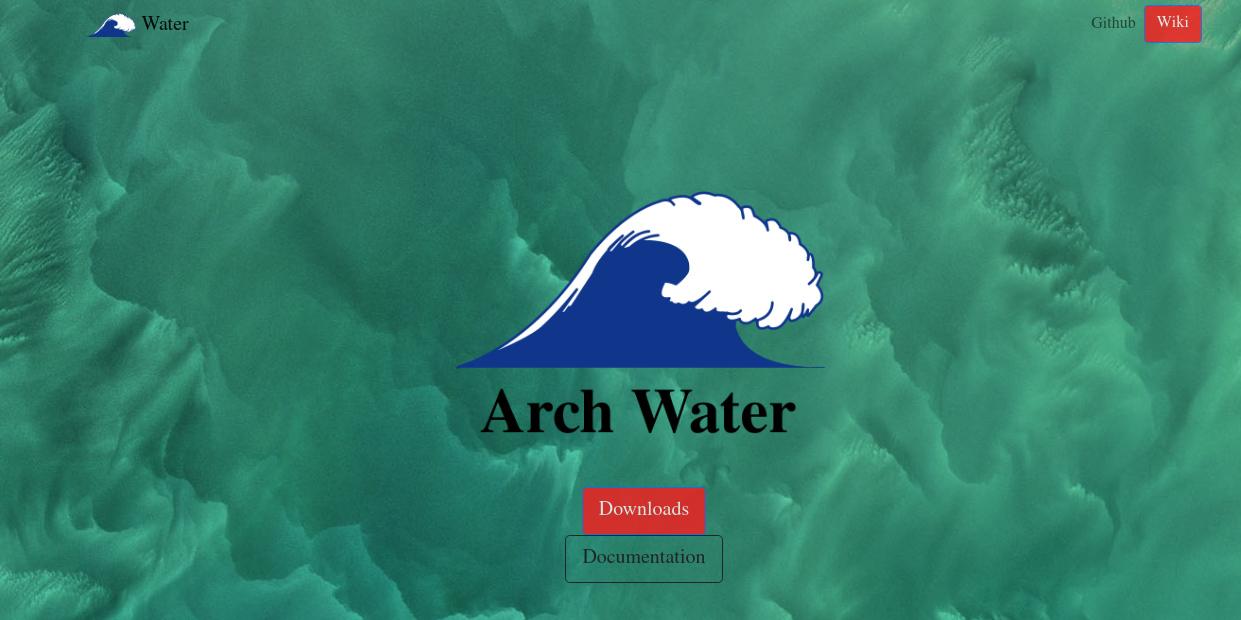
\includegraphics[scale=0.4]{img_presentation/mainPage.png}
			\caption{Pagina principal}
		\end{center}
	\end{figure}


	\begin{figure}[h]
		\begin{center}
			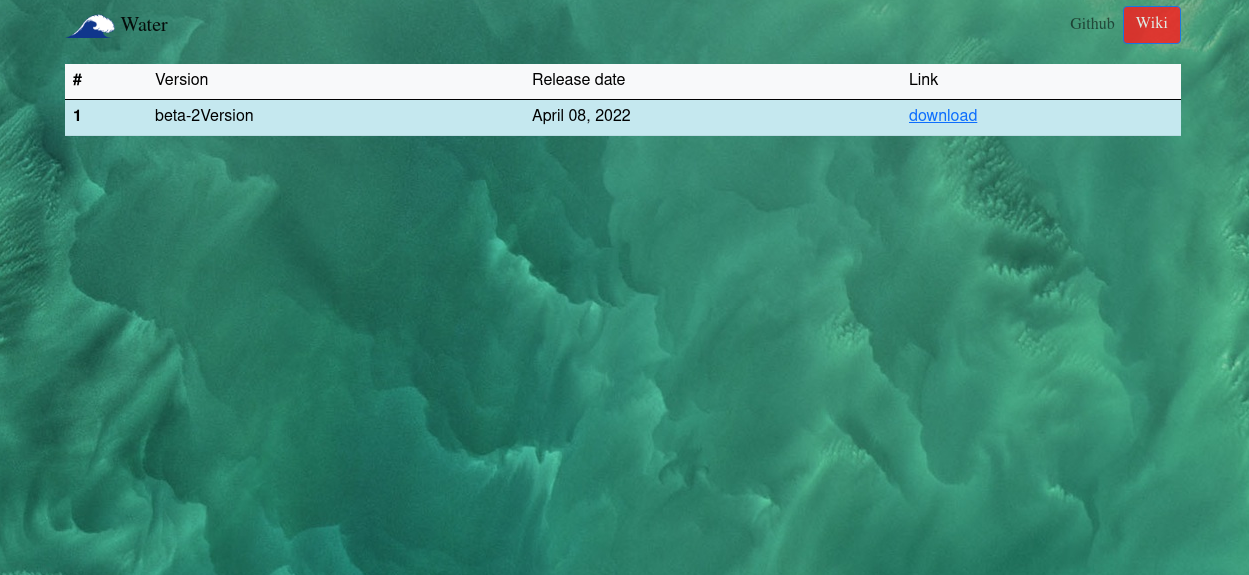
\includegraphics[scale=0.4]{img_presentation/PaginaDeDescargas.png}
			\caption{Pagina de descargas}
		\end{center}
	\end{figure}


\end{section}
\begin{subsection}{Diagramas}
	A continuasion se muestran los diagramas que se pueden usar
	un resumen bastante grande de este es el siguiente diagrama

	\begin{figure}[h]
		\begin{center}
			% incluya aqui la image con \p
			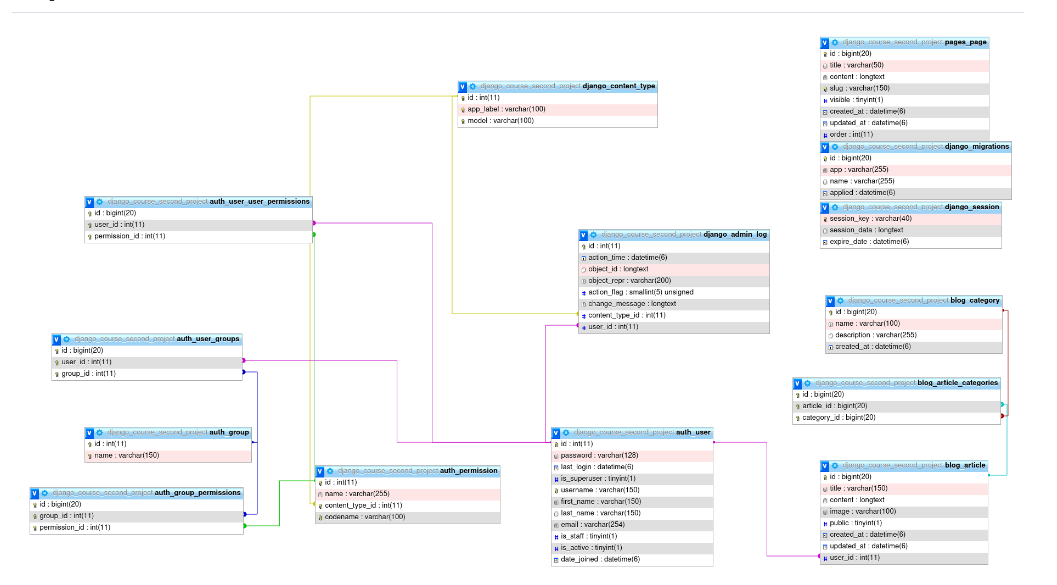
\includegraphics[scale=0.7]{img_presentation/DiagramaBasesDeDatos.png}
			\caption{DiagramaBasesDeDatosCompleto}
		\end{center}
	\end{figure}

	que no se puede ver bastante claro pero en el pdf esta completo


\end{subsection}

\begin{subsection}{codigo de sql}
	el codigo en sql usado para crear las tablas es demasiado extenso pero un
	resumen de como fueron creadas es como este
\begin{minted}{sql}
-- ################################
-- ########## ceated the many to many relationship
-- ################################

CREATE TABLE `Articles_article_categories` (
`id` bigint AUTO_INCREMENT NOT NULL PRIMARY KEY,
`article_id` bigint NOT NULL,
`category_id` bigint NOT NULL
);
-- ################################
-- ########## added the references for the databases
-- ################################

ALTER TABLE `Articles_article`
	ADD CONSTRAINT `Articles_article_user_id_1d4d21bd_fk_auth_user_id`
	FOREIGN KEY (`user_id`) REFERENCES `auth_user` (`id`);

ALTER TABLE `Articles_article_categories`
	ADD CONSTRAINT `Articles_article_categories_article_id_category_id_72321730_uniq`
	UNIQUE (`article_id`, `category_id`);

ALTER TABLE `Articles_article_categories`
	ADD CONSTRAINT `Articles_article_cat_article_id_71d48338_fk_Articles_`
	FOREIGN KEY (`article_id`) REFERENCES `Articles_article` (`id`);


ALTER TABLE `Articles_article_categories`
	ADD CONSTRAINT `Articles_article_cat_category_id_708f65cf_fk_Articles_`
	FOREIGN KEY (`category_id`) REFERENCES `Articles_category` (`id`);

	\end{minted}
\end{subsection}


\end{document}
